\clearpage\setcounter{footnote}{0}
\part{Mathematical Preliminaries}

In this final installment of the paper we
consider the case where the signals or the messages or both are
continuously variable, in contrast with the discrete nature assumed
heretofore.  To a considerable extent the continuous case can be obtained
through a limiting process from the discrete case by dividing the
continuum of messages and signals into a large but finite number of small
regions and calculating the various parameters involved on a discrete
basis.  As the size of the regions is decreased these parameters in general
approach as limits the proper values for the continuous case.  There are,
however, a few new effects that appear and also a general change of
emphasis in the direction of specialization of the general results to
particular cases.

We will not attempt, in the continuous case, to obtain our results with the
greatest generality, or with the extreme rigor of pure mathematics, since
this would involve a great deal of abstract measure theory and would
obscure the main thread of the analysis.  A preliminary study, however,
indicates that the theory can be formulated in a completely axiomatic and
rigorous manner which includes both the continuous and discrete cases and
many others.  The occasional liberties taken with limiting processes in the
present analysis can be justified in all cases of practical interest.

\section{Sets and Ensembles of Functions}

We shall have to deal in the continuous case with sets of functions and
ensembles of functions.  A set of functions, as the name implies, is merely
a class or collection of functions, generally of one variable, time.  It
can be specified by giving an explicit representation of the various
functions in the set, or implicitly by giving a property which functions
in the set possess and others do not.  Some examples are:
\begin{enumerate}
\item
The set of functions:
$$
f_\theta(t)=\sin(t+\theta).
$$
Each particular value of $\theta$ determines a particular function in the
set.
\item
The set of all functions of time containing no frequencies over $W$
cycles per second.
\item
The set of all functions limited in band to $W$ and in amplitude to $A$.
\item
The set of all English speech signals as functions of time.
\end{enumerate}

An \emph{ensemble} of functions is a set of functions together with a
probability measure whereby we may determine the probability of a function
in the set having certain properties.\footnote{In mathematical terminology
the functions belong to a measure space whose total measure is unity.}  For
example with the set,
$$
f_\theta(t)=\sin(t+\theta),
$$
we may give a probability distribution for $\theta$, 
$P(\theta)$.  The set then becomes an ensemble.

Some further examples of ensembles of functions are:
\begin{enumerate}
\item
A finite set of functions $f_k(t)$ ($k=1,2,\dots,n$) with the probability
of $f_k$ being $p_k$.
\item
A finite dimensional family of functions
$$
f(\alpha_1,\alpha_2,\dots,\alpha_n;t)
$$
with a probability distribution on the parameters $\alpha_i$:
$$
p(\alpha_1,\dots,\alpha_n).
$$
For example we could consider the ensemble defined by
$$
f(a_1,\dots,a_n,\theta_1,\dots,\theta_n;t)
	=\sum_{i=1}^n a_i\sin i(\omega t+\theta_i)
$$
with the amplitudes $a_i$ distributed normally and independently, and the
phases $\theta_i$ distributed uniformly (from $0$ to $2\pi$) and
independently.

\item
\label{it:18.3}
The ensemble
$$
f(a_i,t)=\sum_{n=-\infty}^{+\infty} a_n\frac{\sin\pi(2W t-n)}{\pi(2W t-n)}
$$
with the $a_i$ normal and independent all with the same standard deviation
$\sqrt N$.  This is a representation of ``white'' noise, band limited to
the band from $0$ to $W$ cycles per second and with average power
$N$.\footnote{This representation can be used as a definition of band limited
white noise.  It has certain advantages in that it involves fewer limiting
operations than do definitions that have been used in the past.  The name
``white noise,'' already firmly entrenched in the literature, is perhaps
somewhat unfortunate.  In optics white light means either any continuous
spectrum as contrasted with a point spectrum, or a spectrum which is flat
with \emph{wavelength} (which is not the same as a spectrum flat with
frequency).}

\item
\label{it:18.4}
Let points be distributed on the $t$ axis according to a Poisson
distribution.  At each selected point the function $f(t)$ is placed and the
different functions added, giving the ensemble
$$
\sum_{k=-\infty}^\infty f(t+t_k)
$$
where the $t_k$ are the points of the Poisson distribution.  This ensemble
can be considered as a type of impulse or shot noise where all the impulses
are identical.

\item
\label{it:18.5}
The set of English speech functions with the probability measure given by
the frequency of occurrence in ordinary use.
\end{enumerate}

An ensemble of functions $f_\alpha(t)$ is \emph{stationary} if the same
ensemble results when all functions are shifted any fixed amount in time.
The ensemble
$$
f_\theta(t)=\sin(t+\theta)
$$
is stationary if $\theta$ is distributed uniformly from $0$ to $2\pi$.  If
we shift each function by $t_1$ we obtain
\begin{align*}
f_\theta(t+t_1)&=\sin(t+t_1+\theta)\\
	&=\sin(t+\varphi)
\end{align*}
with $\varphi$ distributed uniformly from $0$ to $2\pi$.  Each function has
changed but the ensemble as a whole is invariant under the translation.
The other examples given above are also stationary.

An ensemble is \emph{ergodic} if it is stationary, and there is no subset
of the functions in the set with a probability different from 0 and 1 which
is stationary.  The ensemble
$$
\sin(t+\theta)
$$
is ergodic.  No subset of these functions of probability $\neq0,1$ is
transformed into itself under all time translations.  On the other hand the
ensemble
$$
a\sin(t+\theta)
$$
with $a$ distributed normally and $\theta$ uniform is stationary but not
ergodic.  The subset of these functions with $a$ between 0 and
1 for example is stationary.

Of the examples given, \ref{it:18.3} and \ref{it:18.4} are ergodic, and
\ref{it:18.5} may perhaps be considered so.  If an ensemble is ergodic we
may say roughly that each function in the set is typical of the ensemble.
More precisely it is known that with an ergodic ensemble an average of any
statistic over the ensemble is equal (with probability 1) to an average
over the time translations of a particular function of the
set.\footnote{This is the famous ergodic theorem or rather one aspect of
this theorem which was proved in somewhat different formulations by Birkoff,
von Neumann, and Koopman, and subsequently generalized by Wiener,
Hopf, Hurewicz and others.  The literature on ergodic theory is quite
extensive and the reader is referred to the papers of these writers for
precise and general formulations; e.g., E.~Hopf, ``Ergodentheorie,'' {\it
Ergebnisse der Mathematik und ihrer Grenzgebiete,} v.~5; ``On Causality
Statistics and Probability,'' {\it Journal of Mathematics and Physics,}
v.~XIII, No.~1, 1934; N.~Wiener, ``The Ergodic Theorem,'' {\it Duke
Mathematical Journal,} v.~5, 1939.} Roughly speaking, each function can
be expected, as time progresses, to go through, with the proper frequency,
all the convolutions of any of the functions in the set.

Just as we may perform various operations on numbers or functions to obtain
new numbers or functions, we can perform operations on ensembles to obtain
new ensembles.  Suppose, for example, we have an ensemble of functions
$f_\alpha(t)$ and an operator $T$ which gives for each function
$f_\alpha(t)$ a resulting function $g_\alpha(t)$:
$$
g_\alpha(t)=Tf_\alpha(t).
$$
Probability measure is defined for the set $g_\alpha(t)$ by means of that
for the set $f_\alpha(t)$.  The probability of a certain subset of the
$g_\alpha(t)$ functions is equal to that of the subset of the $f_\alpha(t)$
functions which produce members of the given subset of $g$ functions under
the operation $T$.  Physically this corresponds to passing the ensemble
through some device, for example, a filter, a rectifier or a modulator.
The output functions of the device form the ensemble $g_\alpha(t)$.

A device or operator $T$ will be called invariant if shifting the input
merely shifts the output, i.e., if
$$
g_\alpha(t)=Tf_\alpha(t)
$$
implies
$$
g_\alpha(t+t_1)=Tf_\alpha(t+t_1)
$$
for all $f_\alpha(t)$ and all $t_1$.  It is easily shown (see
Appendix~\ref{ap:5} that if $T$ is invariant
and the input ensemble is stationary then the output ensemble is
stationary.  Likewise if the input is ergodic the output will also be
ergodic.

A filter or a rectifier is invariant under all time translations.  The
operation of modulation is not since the carrier
phase gives a certain time structure.  However, modulation is invariant
under all translations which are multiples of the period of the carrier.

Wiener has pointed out the intimate relation between the invariance of
physical devices under time translations and Fourier
theory.\footnote{Communication theory is heavily indebted to Wiener for
much of its basic philosophy and theory.  His classic NDRC report, {\it The
Interpolation, Extrapolation and Smoothing of Stationary Time Series}
(Wiley, 1949), contains the first clear-cut formulation of communication
theory as a statistical problem, the study of operations on time series.
This work, although chiefly concerned with the linear prediction and
filtering problem, is an important collateral reference in connection with
the present paper.  We may also refer here to Wiener's {\it Cybernetics}
(Wiley, 1948), dealing with the general problems of communication and
control.} He has shown, in fact, that if a device is linear as well as
invariant Fourier analysis is then the appropriate mathematical tool for
dealing with the problem.

An ensemble of functions is the appropriate mathematical representation of
the messages produced by a continuous source (for example, speech), of
the signals produced by a transmitter, and of the perturbing noise.
Communication theory is properly concerned, as has been emphasized by
Wiener, not with operations on particular functions, but with operations on
ensembles of functions.  A communication system is designed not for a
particular speech function and still less for a sine wave, but for the
ensemble of speech functions.

\section{Band Limited Ensembles of Functions}

If a function of time $f(t)$ is limited to the band from $0$ to $W$ cycles
per second it is completely determined by giving its ordinates at a series of
discrete points spaced $\frac1{2W}$ seconds apart in the manner
indicated by the following result.\footnote{For a proof of this theorem and
further discussion see the author's paper ``Communication in the Presence of
Noise'' published in the {\it Proceedings of the Institute of Radio Engineers,}
v.~37, No.~1, Jan., 1949, pp.~10--21.}

\begin{theorem}
\label{thm:13}
Let $f(t)$ contain no frequencies over $W$.  Then
$$
f(t)=\sum_{-\infty}^\infty X_n\frac{\sin\pi(2Wt-n)}{\pi(2Wt-n)}
$$
where
$$
X_n=f\Bigl(\frac{n}{2W}\Bigr).
$$
\end{theorem}

In this expansion $f(t)$ is represented as a sum of orthogonal
functions.  The coefficients $X_n$ of the various terms can be
considered as coordinates in an infinite dimensional  ``function space.''
In this space each function corresponds to precisely one point and each
point to one function.

A function can be considered to be substantially limited to a time $T$
if all the ordinates $X_n$ outside this interval of time are zero.  In
this case all but $2T W$ of the coordinates will be zero.  Thus
functions limited to a band $W$ and duration $T$ correspond to points
in a space of $2T W$ dimensions.

A subset of the functions of band $W$ and duration $T$ corresponds to a
region in this space.  For example, the functions whose total energy is
less than or equal to $E$ correspond to points in a $2T W$ dimensional
sphere with radius $r=\sqrt{2W E}$.

An \emph{ensemble} of functions of limited duration and band will be
represented by a probability distribution $p(x_1,\dots,x_n)$ in the
corresponding $n$ dimensional space.  If the ensemble is not limited in
time we can consider the $2T W$ coordinates in a given interval $T$ to
represent substantially the part of the function in the interval $T$ and
the probability distribution $p(x_1,\dots,x_n)$ to give the statistical
structure of the ensemble for intervals of that duration.

\section{Entropy of a Continuous Distribution}

The entropy of a discrete set of probabilities $p_1,\dots,p_n$ has been
defined as:
$$
H=-\sum p_i\log p_i.
$$
In an analogous manner we define the entropy of a continuous
distribution with the density distribution function $p(x)$ by:
$$
H=-\int_{-\infty}^\infty p(x)\log p(x)\,dx.
$$
With an $n$ dimensional distribution $p(x_1,\dots,x_n)$ we have
$$
H=-\int\dots\int p(x_1,\dots,x_n)\log p(x_1,\dots,x_n)\,
	dx_1\dotsm dx_n.
$$
If we have two arguments $x$ and $y$ (which may themselves be
multidimensional) the joint and conditional entropies of $p(x,y)$ are
given by
\begin{align*}
H(x,y)&=-\iint p(x,y)\log p(x,y)\,dx\,dy\\
\intertext{and}
H_x(y)&=-\iint p(x,y)\log\frac{p(x,y)}{p(x)}\,dx\,dy\\
H_y(x)&=-\iint p(x,y)\log\frac{p(x,y)}{p(y)}\,dx\,dy
\end{align*}
where
\begin{align*}
p(x)&=\int p(x,y)\,dy\\
p(y)&=\int p(x,y)\,dx.
\end{align*}

The entropies of
continuous distributions have most (but not all) of the
properties of the discrete case.  In particular we have the following:
\begin{enumerate}
\item
If $x$ is limited to a certain volume $v$ in its space, then $H(x)$ is a
maximum and equal to $\log v$ when $p(x)$ is constant
($1/v$) in the volume.
\item
With any two variables $x$, $y$ we have
$$
H(x,y)\leq H(x)+H(y)
$$
with equality if (and only if) $x$ and $y$ are independent, i.e.,
$p(x,y)=p(x)p(y)$ (apart possibly from a set of points of probability
zero).
\item
Consider a generalized averaging operation of the following type:
$$
p'(y)=\int a(x,y)p(x)\,dx
$$
with
$$
\int a(x,y)\,dx=\int a(x,y)\,dy=1,\qquad\qquad a(x,y)\geq0.
$$
Then the entropy of the averaged distribution $p'(y)$ is equal to or
greater than that of the original distribution $p(x)$.
\item
We have
\begin{gather*}
H(x,y)=H(x)+H_x(y)=H(y)+H_y(x)\\
\intertext{and}
H_x(y)\leq H(y).
\end{gather*}
\item
Let $p(x)$ be a one-dimensional distribution.  The form of $p(x)$ giving
a maximum entropy subject to the condition that the standard deviation
of $x$ be fixed at $\sigma$ is Gaussian.  To show this we must maximize
$$
H(x)=-\int p(x)\log p(x)\,dx
$$
with
$$
\sigma^2=\int p(x)x^2\,dx\quad\text{and}\quad 1=\int p(x)\,dx
$$
as constraints.  This requires, by the calculus of variations, maximizing
$$
\int\bigl[-p(x)\log p(x)+\lambda p(x)x^2+\mu p(x)\bigr]\,dx.
$$
The condition for this is
$$
-1-\log p(x)+\lambda x^2+\mu=0
$$
and consequently (adjusting the constants to satisfy the constraints)
$$
p(x)=\frac{1}{\sqrt{2\pi}\sigma} e^{-(x^2/2\sigma^2)}.
$$
Similarly in $n$ dimensions, suppose the second order moments of
$p(x_1,\dots,x_n)$ are fixed at $A_{ij}$:
$$
A_{ij}=\int\dots\int x_i x_j p(x_1,\dots,x_n)\,dx_1\dotsm\, dx_n.
$$
Then the maximum entropy occurs (by a similar calculation) when
$p(x_1,\dots,x_n)$ is the $n$ dimensional Gaussian distribution with the
second order moments $A_{ij}$.
\item
The entropy of a one-dimensional Gaussian distribution whose standard
deviation is $\sigma$ is given by
$$
H(x)=\log\sqrt{2\pi e}\sigma.
$$
This is calculated as follows:
\begin{align*}
p(x)&=\frac{1}{\sqrt{2\pi}\sigma}e^{-(x^2/2\sigma^2)}\\
-\log p(x)&=\log\sqrt{2\pi}\sigma+\frac{x^2}{2\sigma^2}\\
H(x)&=-\int p(x)\log p(x)\,dx\\
	&=\int p(x)\log\sqrt{2\pi}\sigma\,dx
		+\int p(x)\frac{x^2}{2\sigma^2}\,dx\\
	&=\log\sqrt{2\pi}\sigma+\frac{\sigma^2}{2\sigma^2}\\
	&=\log\sqrt{2\pi}\sigma+\log\sqrt{e}\\
	&=\log\sqrt{2\pi e}\sigma.
\end{align*}
Similarly the $n$ dimensional Gaussian distribution with associated quadratic
form $a_{ij}$ is given by
$$
p(x_1,\dots,x_n)=\frac{|a_{ij}|^{\frac12}}{(2\pi)^{n/2}}
	\exp\Bigl(-\tfrac12\sum a_{ij} x_i x_j\Bigr)
$$
and the entropy can be calculated as
$$
H=\log(2\pi e)^{n/2}|a_{ij}|^{-\frac12}
$$
where $|a_{ij}|$ is the determinant whose elements are $a_{ij}$.
\item
If $x$ is limited to a half line ($p(x)=0$ for $x\leq0$) and the first
moment of $x$ is fixed at $a$:
$$
a=\int_0^\infty p(x)x\,dx,
$$
then the maximum entropy occurs when
$$
p(x)=\frac1a e^{-(x/a)}
$$
and is equal to $\log ea$.
\item
There is one important difference between the continuous and discrete
entropies.  In the discrete case the entropy measures in an \emph{absolute}
way the randomness of the chance variable.  In the continuous case the
measurement is \emph{relative to the coordinate system}.  If we change
coordinates the entropy will in general change.  In fact if we
change to coordinates $y_1\dotsm y_n$ the new entropy is given by
$$
H(y)=\int\dots\int p(x_1,\dots,x_n)J\Bigl(\frac x y\Bigr)
	\log  p(x_1,\dots,x_n)J\Bigl(\frac x y\Bigr)\,dy_1\dotsm dy_n
$$
where $J\bigl(\frac x y\bigr)$ is the Jacobian of the
coordinate transformation.  On expanding the logarithm and changing the
variables to $x_1\dotsm x_n$, we obtain:
$$
H(y)=H(x)-\int\dots\int p(x_1,\dots,x_n)\log J\Bigl(\frac x y\Bigr)\,
	dx_1\dots dx_n.
$$
Thus the new entropy is the old entropy less the expected logarithm of
the Jacobian.  In the continuous case the entropy can be considered a
measure of randomness \emph{relative to an assumed standard}, namely the
coordinate system chosen with each small volume element $dx_1\dotsm dx_n$
given equal weight.  When we change the coordinate system the entropy in
the new system measures the randomness when equal volume elements
$dy_1\dotsm dy_n$ in the new system are given equal weight.

In spite of this dependence on the coordinate system the entropy concept
is as important in the continuous case as the discrete case.  This is
due to the fact that the derived concepts of information rate and
channel capacity depend on the \emph{difference} of two entropies
and this difference \emph{does not} depend on the coordinate frame, each
of the two terms being changed by the same amount.

The entropy of a continuous distribution can be negative.  The scale of
measurements sets an arbitrary zero corresponding to a uniform
distribution over a unit volume.  A distribution which is more confined
than this has less entropy and will be negative.  The rates and
capacities will, however, always be non-negative.
\item
A particular case of changing coordinates is the linear transformation
$$
y_j=\sum_ia_{ij}x_i.
$$
In this case the Jacobian is simply the determinant $|a_{ij}|^{-1}$ and
$$
H(y)=H(x)+\log|a_{ij}|.
$$
In the case of a rotation of coordinates (or any measure preserving
transformation) $J=1$ and $H(y)=H(x)$.
\end{enumerate}

\section{Entropy of an Ensemble of Functions}

Consider an ergodic ensemble of functions limited to a certain band of
width $W$ cycles per second.  Let
$$
p(x_1,\dots, x_n)
$$
be the density distribution function for amplitudes $x_1,\dots,x_n$ at
$n$ successive sample points.  We define the entropy of the ensemble per
degree of freedom by
$$
H'=-\lim_{n\to\infty}\frac1n\int\dots\int p(x_1,\dots, x_n)
	\log p(x_1,\dots, x_n)\,dx_1\dots dx_n.
$$
We may also define an entropy $H$ per second by dividing, not by $n$,
but by the time $T$ in seconds for $n$ samples.  Since $n=2T W$,
$H=2W H'$.

With white thermal noise $p$ is Gaussian and we have
\begin{align*}
H'&=\log\sqrt{2\pi e N},\\
H&=W\log 2\pi e N.
\end{align*}

For a given average power $N$, white noise has the maximum possible entropy.
This follows from the maximizing properties of the Gaussian distribution
noted above.

The entropy for a continuous stochastic process has many properties
analogous to that for discrete processes.  In the discrete case the
entropy was related to the logarithm of the \emph{probability} of long
sequences, and to the \emph{number} of reasonably probable sequences of
long length.  In the continuous case it is related in a similar fashion
to the logarithm of the \emph{probability density} for a long series of
samples, and the \emph{volume} of reasonably high probability in the
function space.

More precisely, if we assume $p(x_1,\dots,x_n)$ continuous in all the
$x_i$ for all $n$, then for sufficiently large $n$
$$
\Bigl|\frac{\log p}{n}-H'\Bigr|<\eps
$$
for all choices of $(x_1,\dots,x_n)$ apart from a set whose total
probability is less than $\delta$, with $\delta$ and $\eps$ arbitrarily
small.  This follows form the ergodic property if we divide the space
into a large number of small cells.

The relation of $H$ to volume can be stated as follows:  Under the same
assumptions consider the $n$ dimensional space corresponding to
$p(x_1,\dots,x_n)$.  Let $V_n(q)$ be the smallest volume in this space
which includes in its interior a total probability $q$.  Then
$$
\lim_{n\to\infty}\frac{\log V_n(q)}{n}=H'
$$
provided $q$ does not equal 0 or 1.

These results show that for large $n$ there is a rather well-defined
volume (at least in the logarithmic sense) of high probability, and that
within this volume the probability density is relatively uniform (again
in the logarithmic sense).

In the white noise case the distribution function is given by
$$
p(x_1,\dots,x_n)=\frac{1}{(2\pi N)^{n/2}}\exp -\frac{1}{2N}\sum x_i^2.
$$
Since this depends only on $\sum x_i^2$ the surfaces of equal
probability density are spheres and the entire distribution has spherical
symmetry.  The region of high probability is a sphere of radius $\sqrt{n
N}$.  As $n\to\infty$ the probability of being outside a sphere of
radius $\sqrt{n(N+\eps)}$ approaches zero and
$\frac1n$ times the logarithm of the volume of the sphere
approaches $\log\sqrt{2\pi e N}$.

In the continuous case it is convenient to work not with the entropy $H$
of an ensemble but with a derived quantity which we will call the
entropy power.  This is defined as the power in a white noise
limited to the same band as the original ensemble and having the same
entropy.  In other words if $H'$ is the entropy of an ensemble its
entropy power is
$$
N_1=\frac{1}{2\pi e}\exp 2H'.
$$
In the geometrical picture this amounts to measuring the high
probability volume by the squared radius of a sphere having the same
volume.  Since white noise has the maximum entropy for a given power,
the entropy power of any noise is less than or equal to its actual
power.

\section{Entropy Loss in Linear Filters}

\begin{table}[ht]
\caption{}
\label{tab:1}
\tabcolsep=2pt
\footnotesize
\centerline{\begin{tabular}{|c|c|c|c|}
\hline
& \sc entropy & \sc entropy &\\[-.8ex]
\sc gain & \sc power & \sc power gain & \sc impulse response\\[-.8ex]
& \sc factor & \sc in decibels &\\
\hline
\begin{picture}(0,0)%

\epsfig{file=tab1a.ps}%
\end{picture}%
\setlength{\unitlength}{1bp}%
\begin{picture}(120,70)
\put(55,3){\makebox(0,0){\sf 0}}
\put(115,3){\makebox(0,0){\sf 1}}
\put(85,3){\makebox(0,0){$\omega$}}
\put(50,63){\makebox(0,0){\sf 1}}
\put(30,38){\makebox(0,0)[r]{$1-\omega$}}
\end{picture}
 &
   \raisebox{30bp}{$\displaystyle\frac{1}{e^2}$} &
   \raisebox{30bp}{$-8.69$} &
   \raisebox{30bp}{$\displaystyle
		\frac{\sin^2(t/2)}{t^2/2}$}\\
\hline
\begin{picture}(0,0)%

\epsfig{file=tab1b.ps}%
\end{picture}%
\setlength{\unitlength}{1bp}%
\begin{picture}(120,70)
\put(55,3){\makebox(0,0){\sf 0}}
\put(115,3){\makebox(0,0){\sf 1}}
\put(85,3){\makebox(0,0){$\omega$}}
\put(50,63){\makebox(0,0){\sf 1}}
\put(30,38){\makebox(0,0)[r]{$1-\omega^2$}}
\end{picture}
 &
   \raisebox{30bp}{$\displaystyle\Bigl(\frac{2}{e}\Bigr)^4$} &
   \raisebox{30bp}{$-5.33$} &
   \raisebox{30bp}{$\displaystyle
       2\left[\frac{\sin t}{t^3}-\frac{\cos t}{t^2}\right]$} \\
\hline
\begin{picture}(0,0)%
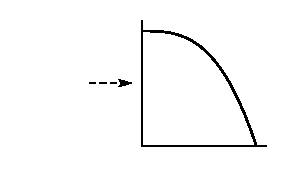
\epsfig{file=tab1c.ps}%
\end{picture}%
\setlength{\unitlength}{1bp}%
\begin{picture}(120,70)
\put(55,3){\makebox(0,0){\sf 0}}
\put(115,3){\makebox(0,0){\sf 1}}
\put(85,3){\makebox(0,0){$\omega$}}
\put(50,63){\makebox(0,0){\sf 1}}
\put(30,38){\makebox(0,0)[r]{$1-\omega^3$}}
\end{picture}
 &
   \raisebox{30bp}{$0.411$} &
   \raisebox{30bp}{$-3.87$} &
   \raisebox{30bp}{$\displaystyle
      6\left[\frac{\cos t-1}{t^4}-\frac{\cos t}{2t^2}
      +\frac{\sin t}{t^3}\right]$} \\
\hline
\begin{picture}(0,0)%
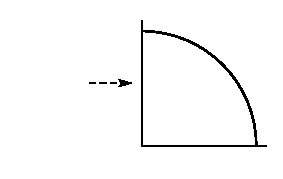
\epsfig{file=tab1d.ps}%
\end{picture}%
\setlength{\unitlength}{1bp}%
\begin{picture}(120,70)
\put(55,3){\makebox(0,0){\sf 0}}
\put(115,3){\makebox(0,0){\sf 1}}
\put(85,3){\makebox(0,0){$\omega$}}
\put(50,63){\makebox(0,0){\sf 1}}
\put(32,38){\makebox(0,0)[r]{$\sqrt{1-\omega^2}$}}
\end{picture}
 &
   \raisebox{30bp}{$\displaystyle\Bigl(\frac{2}{e}\Bigr)^2$} &
   \raisebox{30bp}{$-2.67$} &
   \raisebox{30bp}{$\displaystyle \frac{\pi}{2}\frac{J_1(t)}{t}$} \\
\hline
\begin{picture}(0,0)%
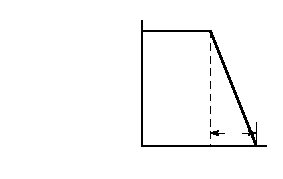
\epsfig{file=tab1e.ps}%
\end{picture}%
\setlength{\unitlength}{1bp}%
\begin{picture}(120,70)
\put(55,3){\makebox(0,0){\sf 0}}
\put(115,3){\makebox(0,0){\sf 1}}
\put(85,3){\makebox(0,0){$\omega$}}
\put(50,63){\makebox(0,0){\sf 1}}
\put(104,14){\makebox(0,0){$\alpha$}}
\end{picture}
 &
   \raisebox{30bp}{$\displaystyle\frac{1}{e^{2\alpha}}$} &
   \raisebox{30bp}{$-8.69\alpha$} &
   \raisebox{30bp}{$\displaystyle
      \frac{1}{\alpha t^2}\bigl[\cos(1-\alpha)t-\cos t\bigr]$} \\
\hline
\end{tabular}}
\end{table}

\begin{theorem}
\label{thm:14}
If an ensemble having an entropy $H_1$ per degree of freedom in band $W$ is
passed through a filter with characteristic $Y(f)$ the output ensemble has
an entropy
$$
H_2=H_1+\frac1W\int_W \log|Y(f)|^2\,df.
$$
\end{theorem}

The operation of the filter is essentially a linear transformation
of coordinates.  If we think of the different frequency components as the
original coordinate system, the new frequency components are merely the old
ones multiplied by factors.  The coordinate transformation matrix is thus
essentially diagonalized in terms of these coordinates.  The Jacobian of
the transformation is (for $n$ sine and $n$ cosine components)
$$
J=\prod_{i=1}^n|Y(f_i)|^2
$$
where the $f_i$ are equally spaced through the band $W$.  This becomes in
the limit
$$
\exp\frac1W\int_W\log|Y(f)|^2\,df.
$$
Since $J$ is constant its average value is the same quantity and applying
the theorem on the change of entropy with a change of coordinates, the
result follows.  We may also phrase it in terms of the entropy power.
Thus if the entropy power of the first ensemble is $N_1$ that of the second
is
$$
N_1\exp\frac1W\int_W\log|Y(f)|^2\,df.
$$
The final entropy power is the initial entropy power multiplied by the
geometric mean gain of the filter.  If the gain is measured in {\it db},
then the output entropy power will be increased by the arithmetic mean {\it
db} gain over $W$.

In Table~\ref{tab:1} the entropy power loss has been calculated (and also
expressed in {\it db}) for a number of ideal gain characteristics.  The
impulsive responses of these filters are also given for $W=2\pi$, with
phase assumed to be $0$.

The entropy loss for many other cases can be obtained from these results.
For example the entropy power factor $1/e^2$ for the
first case also applies to any gain characteristic obtain from $1-\omega$
by a measure preserving transformation of the $\omega$ axis.  In particular
a linearly increasing gain $G(\omega)=\omega$, or a ``saw tooth''
characteristic between 0 and 1 have the same entropy loss.  The reciprocal
gain has the reciprocal factor.  Thus $1/\omega$ has the
factor $e^2$.  Raising the gain to any power raises the factor to this power.

\section{Entropy of a Sum of Two  Ensembles}

If we have two ensembles of functions $f_\alpha(t)$ and $g_\beta(t)$ we can
form a new ensemble by ``addition.''  Suppose the first ensemble has the
probability density function $p(x_1,\dots,x_n)$ and the second
$q(x_1,\dots,x_n)$.  Then the density function for the sum is given by the
convolution:
%\begin{multline*}
$$
r(x_1,\dots,x_n)=\int\dots\int p(y_1,\dots,y_n) %\\ \cdot
q(x_1-y_1,\dots,x_n-y_n)\,dy_1\dotsm dy_n.
$$
%\end{multline*}
Physically this corresponds to adding the noises or signals represented by
the original ensembles of functions.

The following result is derived in Appendix~\ref{ap:6}.
\begin{theorem}
\label{thm:15}
Let the average power of two ensembles be $N_1$ and $N_2$ and let their
entropy powers be $\overline N_1$ and $\overline N_2$.  Then the entropy
power of the sum, $\overline N_3$, is bounded by
$$
\overline N_1+\overline N_2\leq\overline N_3\leq N_1+N_2.
$$
\end{theorem}

White Gaussian noise has the peculiar property that it can absorb any other
noise or signal ensemble which may be added to it with a resultant entropy
power approximately equal to the sum of the white noise power and the signal
power (measured from the average signal value, which is normally zero),
provided the signal power is small, in a certain sense, compared to noise.

Consider the function space associated with these ensembles having $n$
dimensions.  The white noise corresponds to the spherical Gaussian
distribution in this space.  The signal ensemble corresponds to another
probability distribution, not necessarily Gaussian or spherical.  Let the
second moments of this distribution about its center of gravity be
$a_{ij}$.  That is, if $p(x_1,\dots,x_n)$ is the density distribution
function
$$
a_{ij}=\int\dots\int p(x_i-\alpha_i)(x_j-\alpha_j)\,dx_1\dotsm dx_n
$$
where the $\alpha_i$ are the coordinates of the center of gravity.  Now
$a_{ij}$ is a positive definite quadratic form, and we can rotate our
coordinate system to align it with the principal directions of this form.
$a_{ij}$ is then reduced to diagonal form $b_{ii}$.  We require that each
$b_{ii}$ be small compared to $N$, the squared radius of the spherical
distribution.

In this case the convolution of the noise and signal produce approximately
a Gaussian distribution whose corresponding quadratic form is
$$
N+b_{ii}.
$$
The entropy power of this distribution is
$$
\Bigl[\prod(N+b_{ii})\Bigr]^{1/n}
$$
or approximately
\begin{gather*}
=\Bigl[(N)^n+\sum b_{ii}(N)^{n-1}\Bigr]^{1/n}\\
\doteq N+\frac1n\sum b_{ii}.
\end{gather*}
The last term is the signal power, while the first is the noise power.

